\section{Results}
\label{sec:results}

The full set of data from 2016, 2017, and 2018 in all selection categories
is tested against multiple $\HH$ production hypotheses,
described in Section~\ref{sec:introduction}: the Standard Model prediction;
variations of the SM coupling constant modifiers
$\kappal$, $\kappat$, $\kappaV$, $\kappaVV$, and [TODO 5th?];
BSM effective couplings $\cg$, $\cgg$, and $\ctwo$;
and resonant production from the decay of spin-0 or
spin-2 particles with masses between 250 and $1000\GeV$.
In each case, the entire dataset is fit simultaneously to a model
composed of the background prediction (with uncertainties),
and the $\HH$ signal hypothesis under consideration.

The SM ``signal strength'' parameter is defined as
$\mu = \sigma(\HH)_{\textrm{best fit}} / \sigma(\HH)_{\textrm{SM}}$,
and modifies the expected signal yield by the same proportion in each category.
By contrast, variations in the $\kappa$ modifiers affect the signal yields in each
category separately, and change the BDT discriminant output shape for $\HH$ events.
The twelve benchmark scenarios spanning combinations of $\kappal$, $\kappat$,
$\cg$, $\cgg$, and $\ctwo$ values in the EFT phase space each correspond to
different signal kinematics, so the $\HH$ production cross section $\sigma$
for each point is measured separately.
Similarly, signal efficiency and BDT output vary dramatically for different
resonant masses, so each mass and spin hypothesis gets a discrete measurement.
The SM signal strength and $\kappa$ measurements are performed with $\ggHH$ and
$\qqHH$ signal MC simulation generated at NLO, using the SM ``node'' of the BDT
training in each event category to produce the final disciminator output distribution.
Each EFT point and resonant hypothesis has its own dedicated BDT node, and
is measured using a unique BDT output distribution in LO $\ggHH$ MC simulation.
[TODO: describe choice of BDT binning.]

The SM signal strength is measured using a profile likelihood test
statistic~\cite{Cowan:2010js}, with systematic uncertainties treated as nuisance
parameters $\theta$ in a modified frequentist approach.~\cite{ATL-PHYS-PUB-2011-011}
The likelihood ratio $q_{\mu}$ for a fixed ``test'' signal strength value $\mu$ is:

\begin{linenomath}
\begin{equation*}
  \begin{aligned}
    q_{\mu}  &  = -2 \Delta \ln \mathcal{L} = \ln \frac{\mathcal{L}(\mathrm{data}|\mu,\hat{\theta}_{\mu})}{\mathcal{L}(\mathrm{data}|\hat{\mu},\hat{\theta})}
  \end{aligned}
\end{equation*}
\end{linenomath}

where $\hat{\mu}$ and $\hat{\theta}$ are the signal strength and nuisance
paramter values which give the maximum value of likelihood $\mathcal{L}$
for the given set of data, and $\hat{\theta}_{\mu}$ is the set of nuisance
parameter values which maximize $\mathcal{L}$ for the fixed $\mu$ value.
The 95\% confidence interval includes all values of $\mu$ for which $q_{\mu} < 1.96$,
within approximately 2 standard deviations of the global best-fit value ($q_{\mu} = 0$).
The SM coupling strength modifiers and and BSM scenario cross sections
are measured by profiling values of $\kappa$ and $\sigma$, respectively,
relative to $\hat{\kappa}$ and $\hat{\sigma}$.
Theoretical and experimental uncertainties affecting the signal and
background yields or discriminator output distributions are fully
correlated across all years, event categories, and discriminant bins,
except as noted in Section~\ref{sec:systematicUncertainties}.

The fits to all BDT output ``node'' distributions in data are consistent with the
SM background prediction in all selection categories, within systematic uncertainties.
The observed 95\% CL upper limit on the SM $\HH$ production cross section
from data is X.XX~\pb (Y.YY times the SM prediction), compared to an
expected limit of Z.ZZ~\pb in the absence of $\HH$ signal events.
These limits are shown in Fig.~\ref{fig:HH_limits_SM} [TODO: Create],
for individual categories as well as the combined result.
The \lttt and \lllnot categories providethe strongest individual
constraints on the SM $\HH$ cross section.

\begin{figure}
  \centering
  %% \includegraphics[width=0.45\textwidth]{figures/SM_limits.pdf}
  \caption{
    Observed and expected 95\% CL limits on the SM $\HH$ production cross section
    for the CMS Run~2 dataset of 137.2\fbinv, for both individual event categories
    and their combination.
  }
  \label{fig:HH_limits_SM}
\end{figure}

The 95\% CL interval for the Higgs boson trilinear self-coupling strength modifier
is measured to be $X.XX < \kappal < Y.YY$, where the upper limit is the [second]
strongest constraint on this fundamental SM parameter to date.~\cite{Sirunyan:2745738,Sirunyan:2018ayu,2020135103}
%% CMS Run 2 bbgg limits -3.3 to 8.5, combined 2016 limits -11.8 to 18.8
%% ATLAS combined 2016 limits -5.0 to 12.0
The observed and expected upper limits on the $\HH$ production cross section as a function of
$\kappal$ are shown in Fig.~\ref{fig:HH_limits_kLambda}, along with limits for each event category.
%% Some comment on strongest limits near max/min kLambda values

\begin{figure}
  \centering
  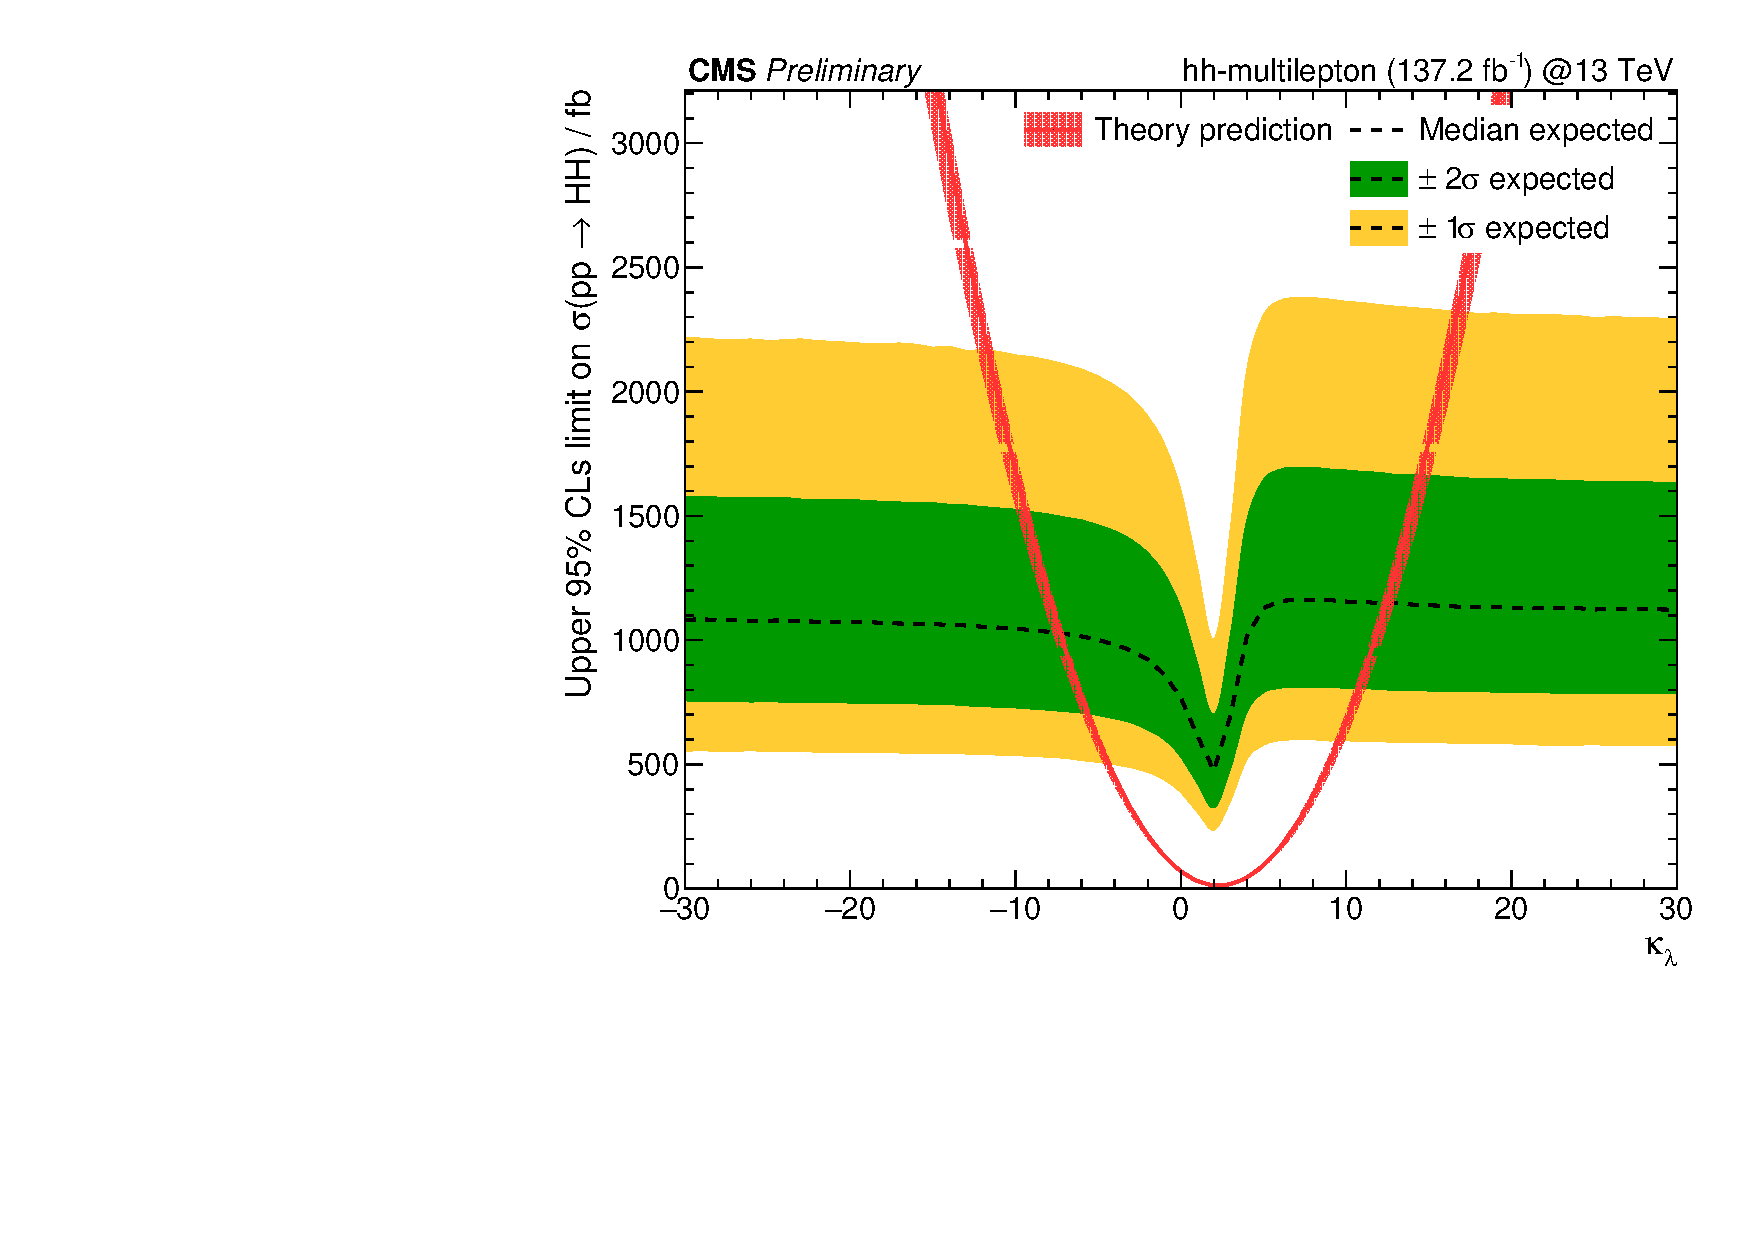
\includegraphics[width=0.45\textwidth]{figures/klscan.pdf}
  \hspace{0.05\textwidth}
  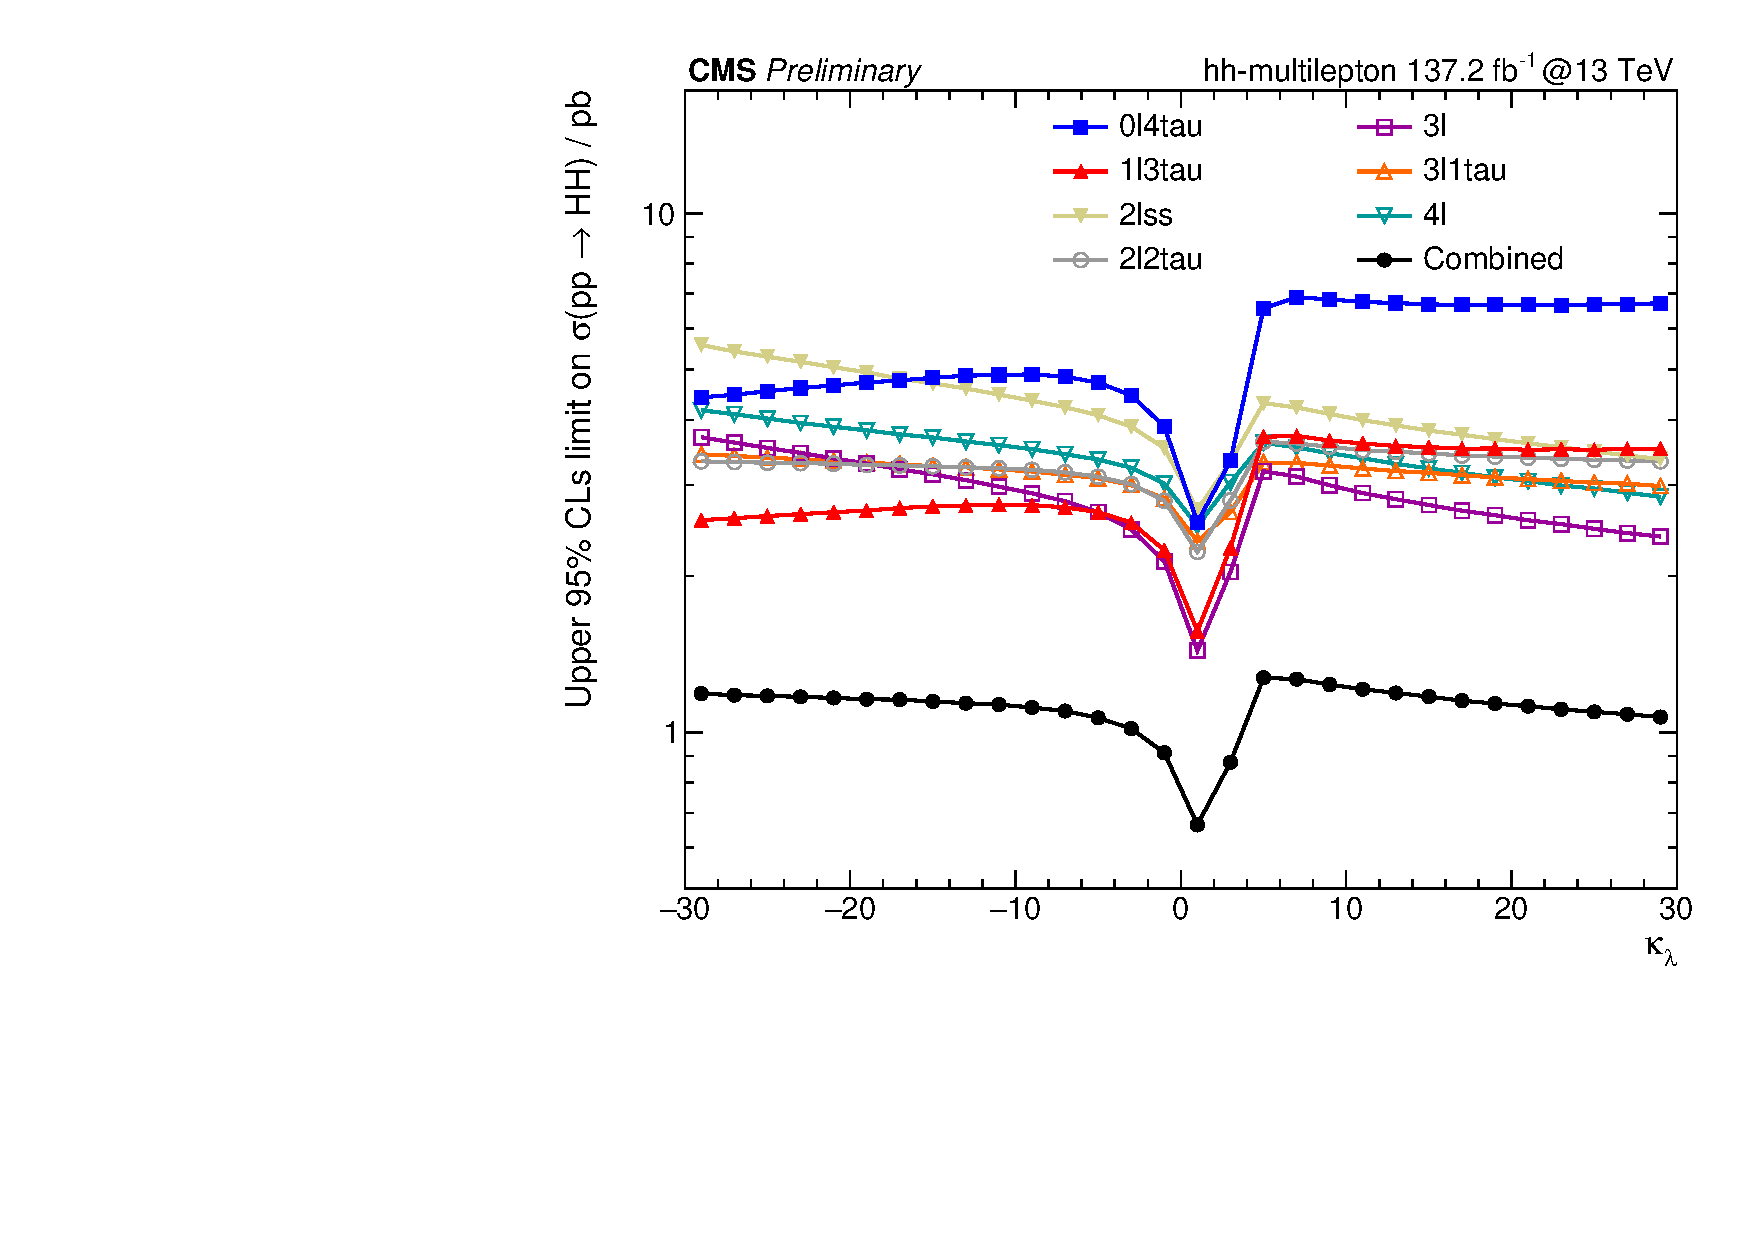
\includegraphics[width=0.45\textwidth]{figures/klMultiscan.pdf}
  \caption{
    Observed and expected 95\% CL limits on the $\HH$ production cross section as
    a function of the Higgs boson self-coupling strength modidifier $\kappal$.
    The plot on the left shows the combined result with all event categories for
    the CMS Run~2 dataset of 137.2\fbinv, while the plot on the right shows the
    seven event categories separately.  Overlaid is a curve representing the
    predicted $\HH$ production cross section if all SM constants other than
    $\lambda$ have the values predicted in the SM.
  }
  \label{fig:HH_limits_kLambda}
\end{figure}

Observed and expected limits on the $\HH$ production cross section in
twelve EFT benchmark scenarios are shown in Fig.~\ref{fig:HH_limits_EFT}
and summarized in Table~TODO.
For benchmarks X, Y, and Z, the upper limit cross sections are lower
than for any previous measurement.~\cite{Sirunyan:2745738}
These benchmarks represent models in which the $\HH$ invariant mass is
lower than the SM prediction.  This analysis has higher signal efficiency
in the low-mass phase space relative to searches with at least one Higgs decay
to bottom quarks because electrons and muons with $\pt < 30\GeV$ have higher
reconstruction and identification efficiency than low-$\pt$ hadronic jets in CMS.

\begin{figure}
  \centering
  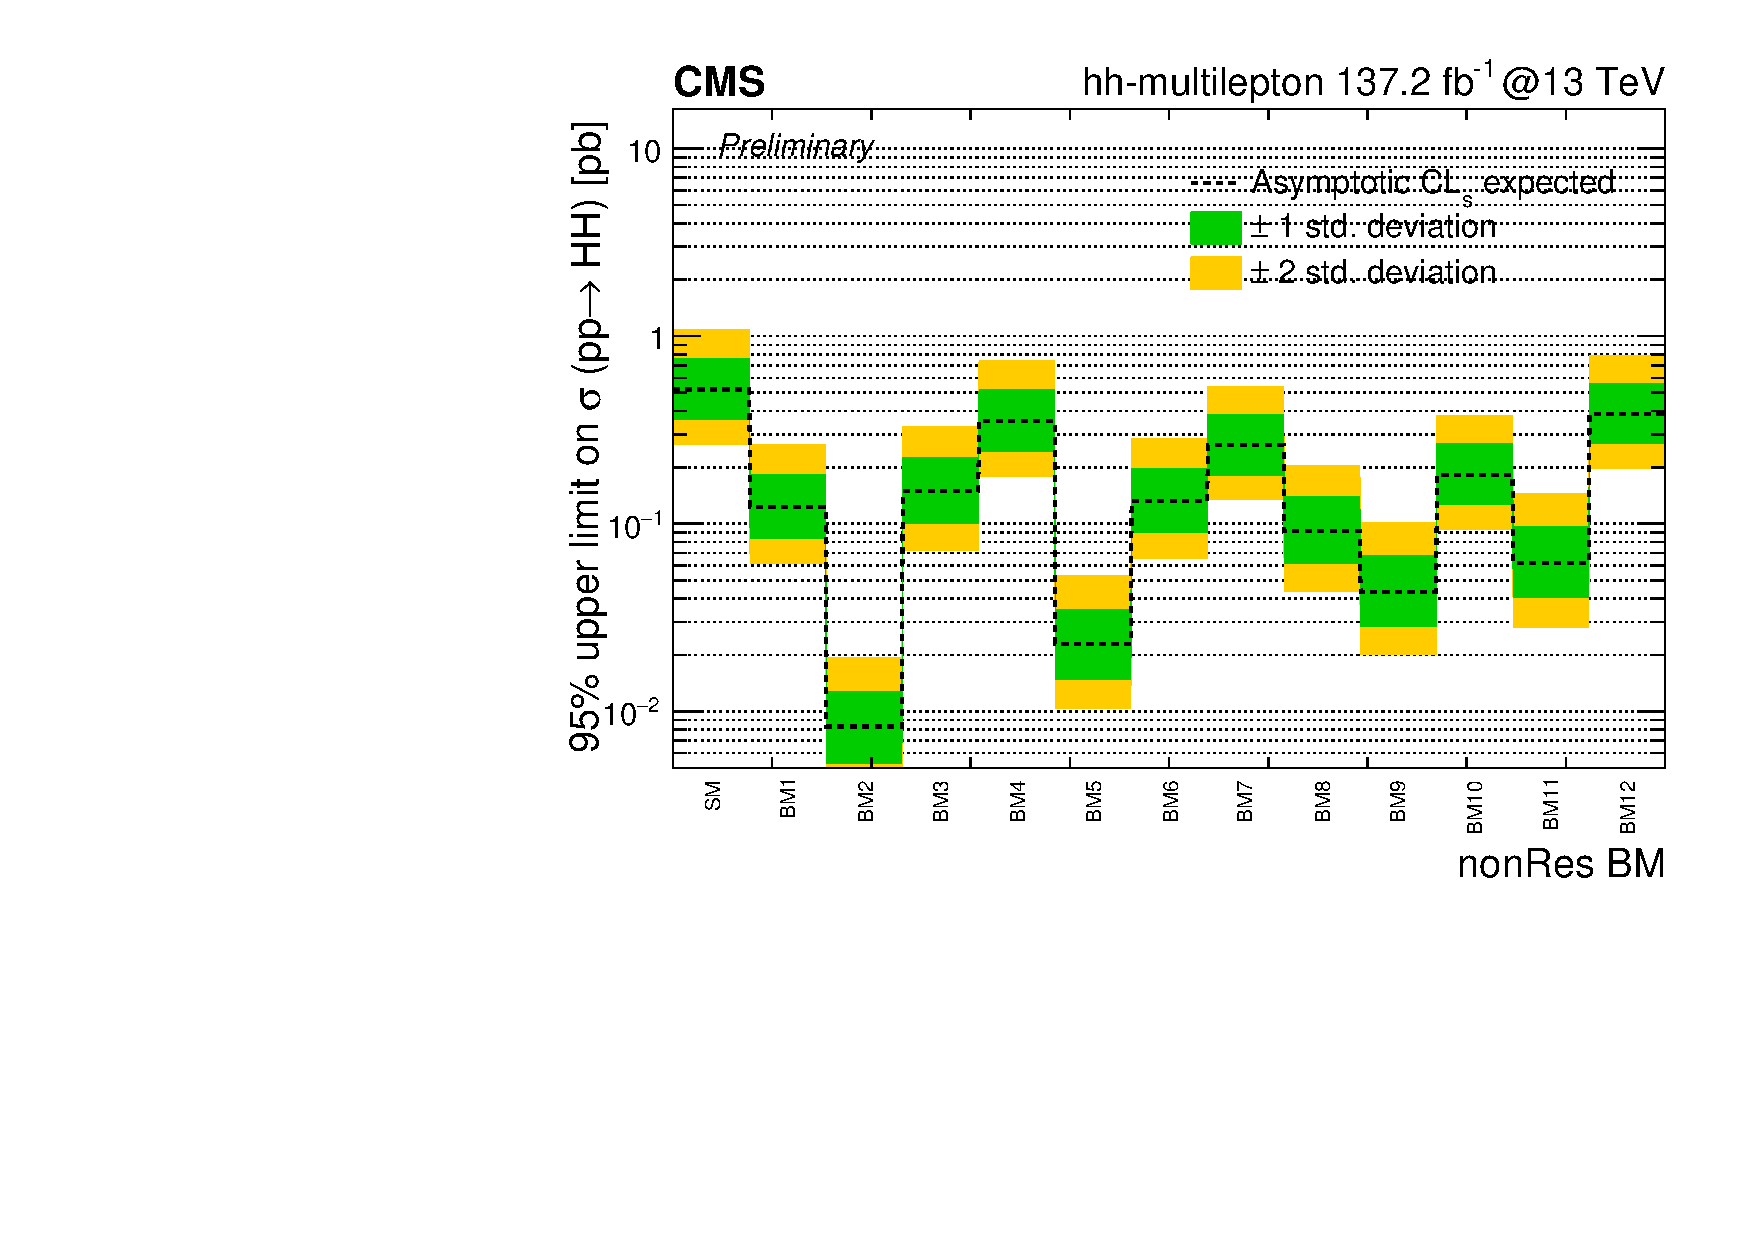
\includegraphics[width=0.45\textwidth]{figures/bmScan_multilepton_RUN2.pdf}
  \hspace{0.05\textwidth}
  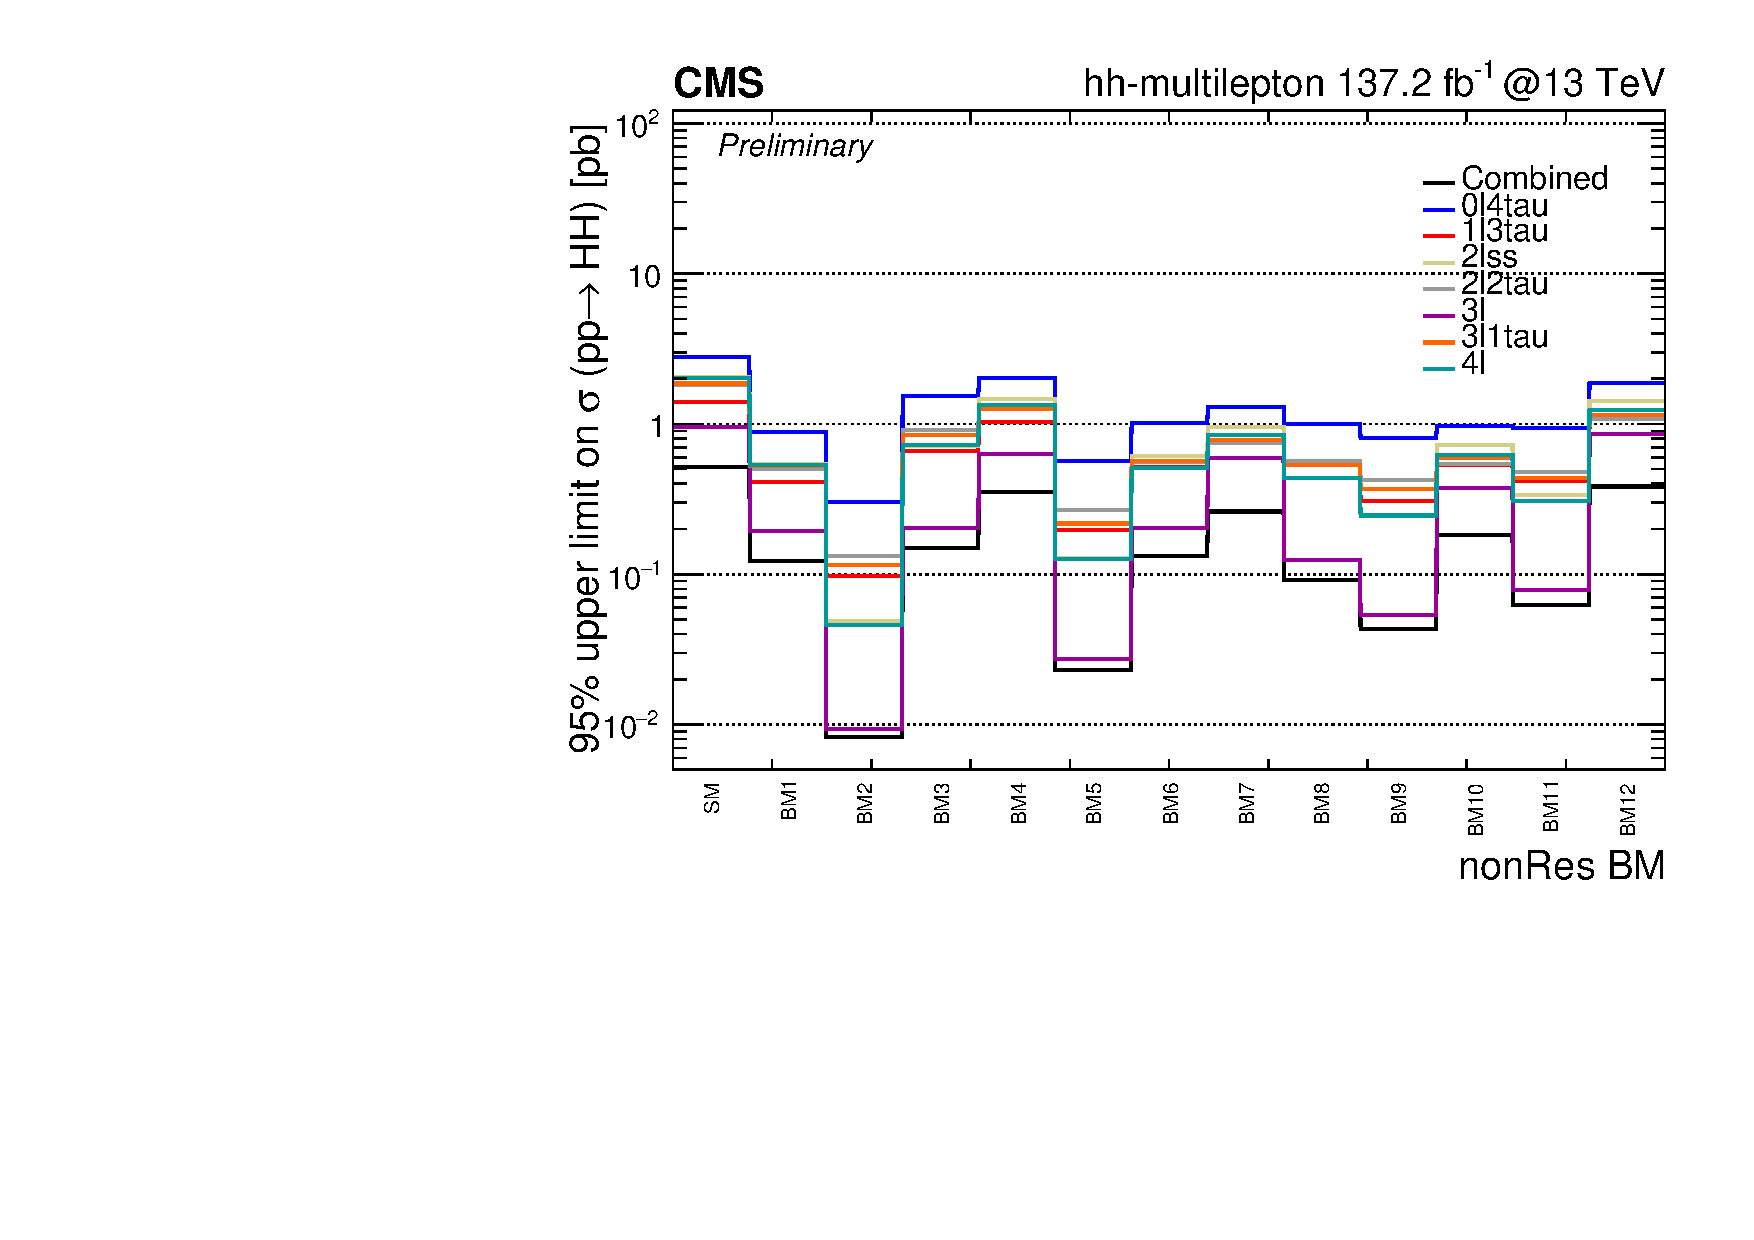
\includegraphics[width=0.45\textwidth]{figures/multiBMScan_multilepton_Run2.pdf}
  \caption{
    Observed and expected 95\% CL limits on the $\HH$ production cross section for
    twelve EFT benchmark scenarios as well the SM, modeled at LO in MC simulation.
    The plot on the left shows the combined result with all event categories for
    the CMS Run~2 dataset of 137.2\fbinv, while the plot on the right shows the
    seven event categories separately.
  }
  \label{fig:HH_limits_EFT}
\end{figure}

Figures~\ref{fig:HH_limits_spin0} and \ref{fig:HH_limits_spin2} show observed and
expected limits on the resonant $\HH$ production cross section as a function of
$\HH$ invariant mass, for spin-0 and spin-2 particles decaying to a Higgs pair.
Compared to previously published searches for resonant $\HH$
production~\cite{Sirunyan:2018ayu,2020135103},
this result has similar sensitivity at very low masses ($250 - 400\GeV$),
again thanks to the superior CMS reconstruction of low-$\pt$ leptons.

\begin{figure}
  \centering
  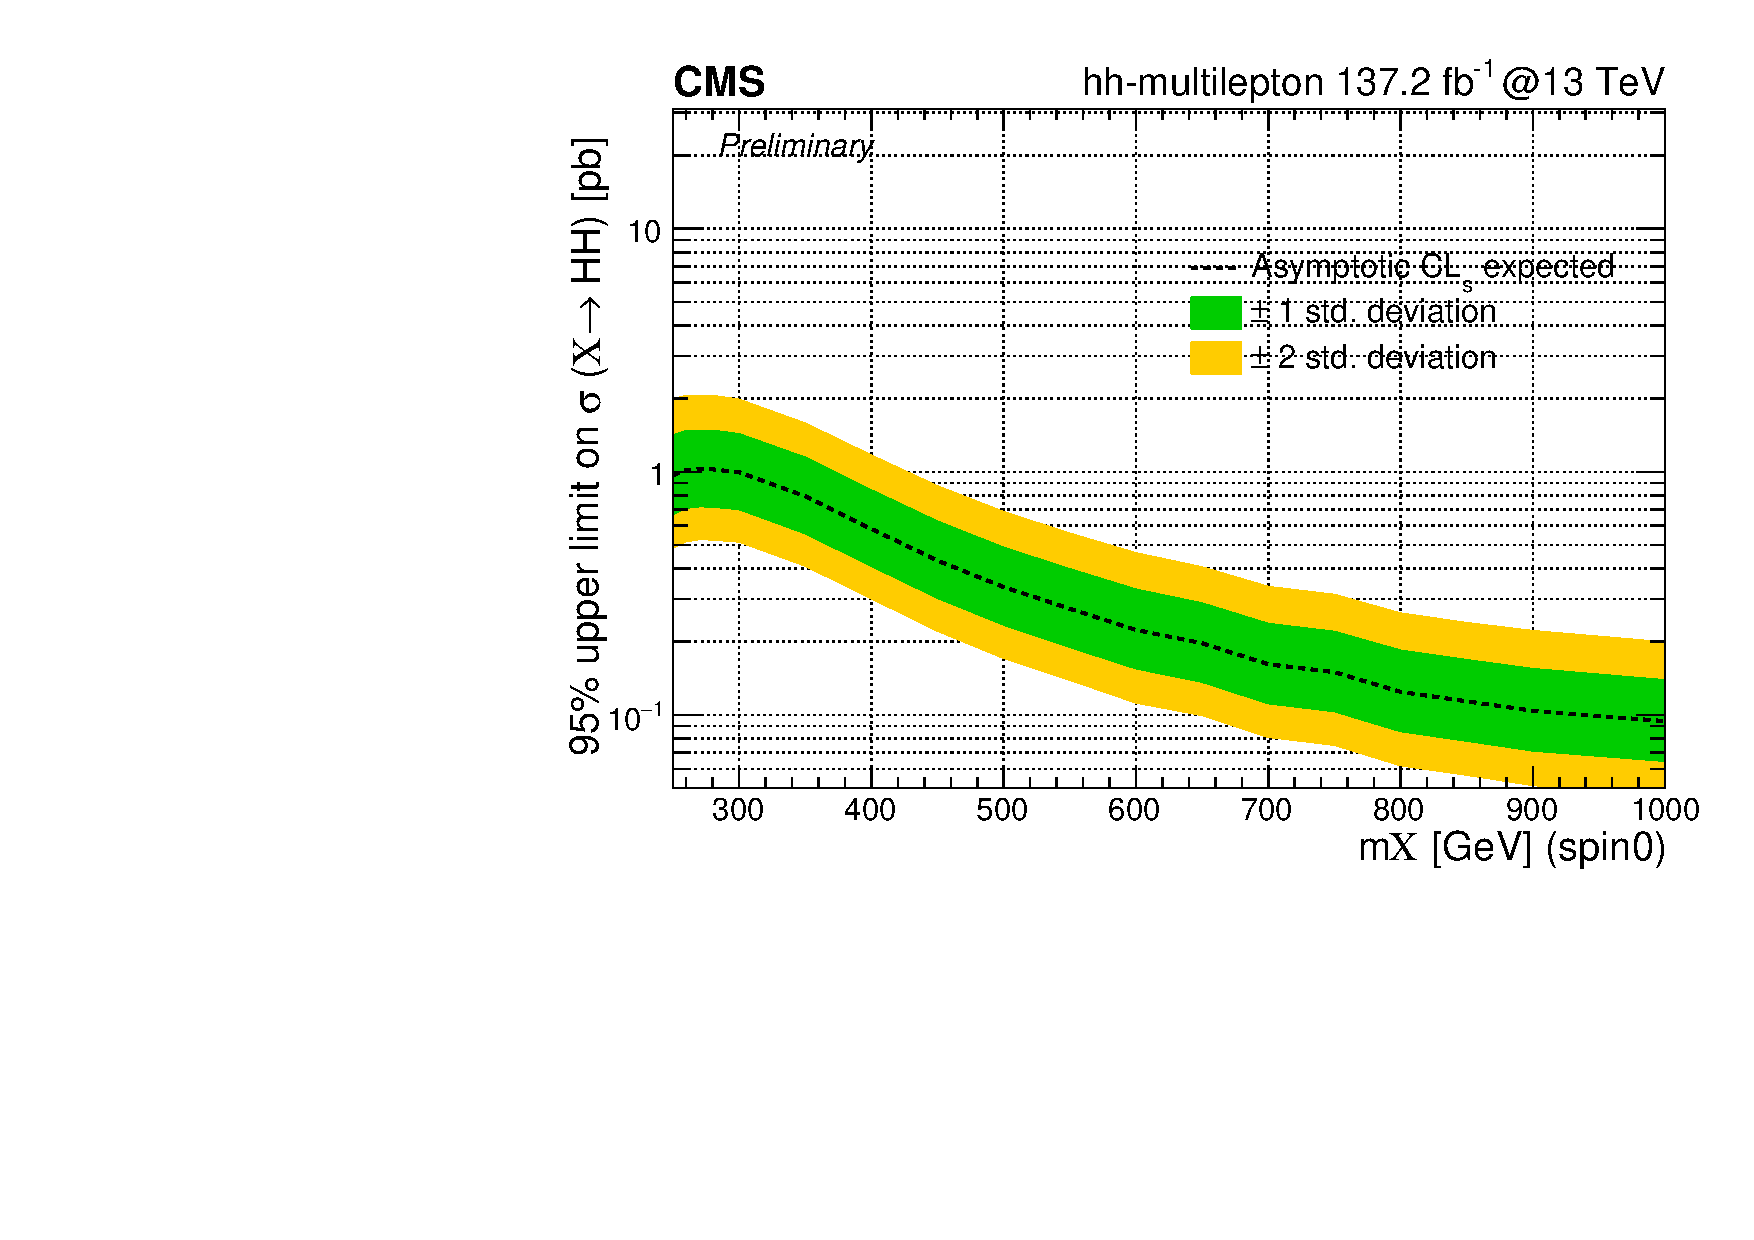
\includegraphics[width=0.45\textwidth]{figures/massScan_spin0_multilepton_RUN2.pdf}
  \hspace{0.05\textwidth}
  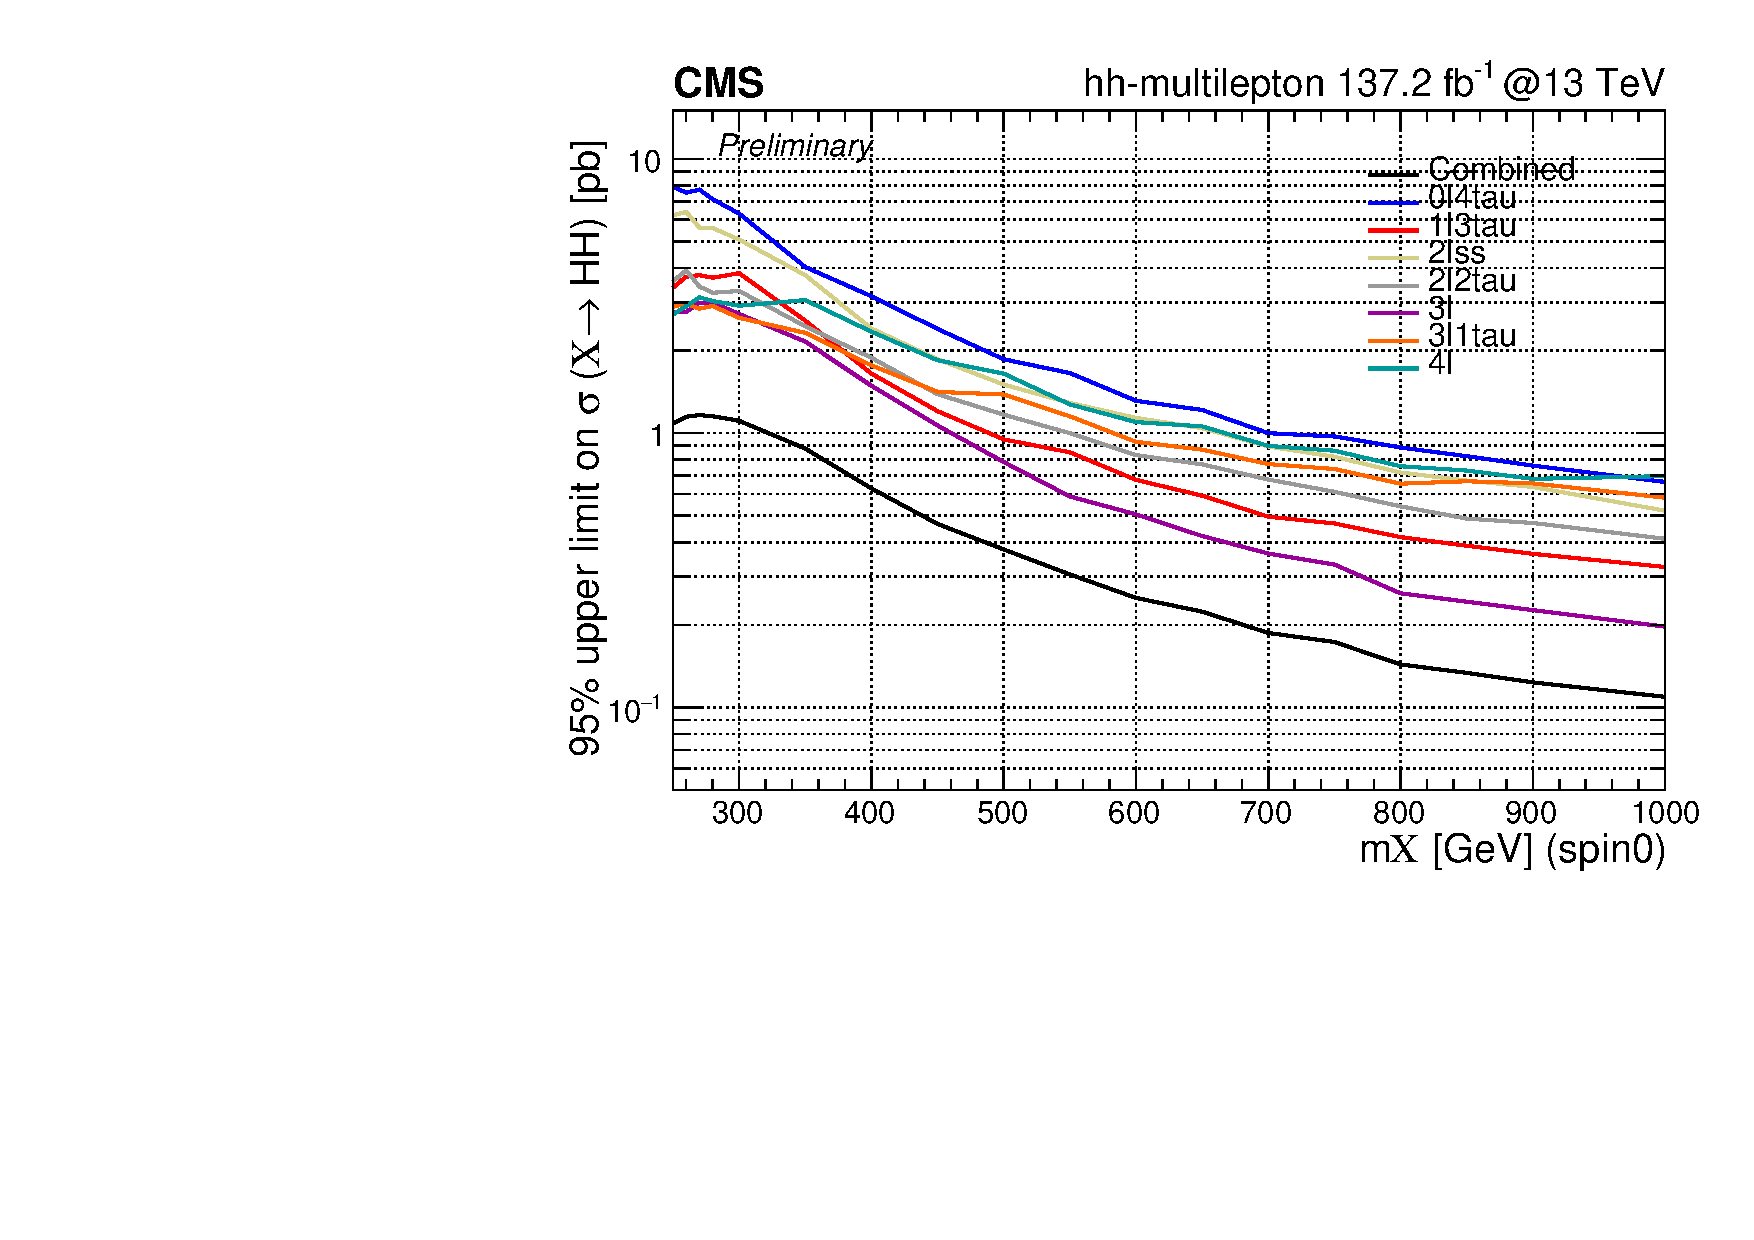
\includegraphics[width=0.45\textwidth]{figures/massMultiScan_spin0_multilepton_Run2.pdf}
  \caption{
    Observed and expected 95\% CL limits on resonant spin-0 $\HH$ production in
    the mass range $250 - 1000\GeV$ for the CMS Run~2 dataset of 137.2\fbinv,
    for the combination of all event categories (left),
    and for each of the seven event categories separately (right).
  }
  \label{fig:HH_limits_spin0}
\end{figure}

\begin{figure}
  \centering
  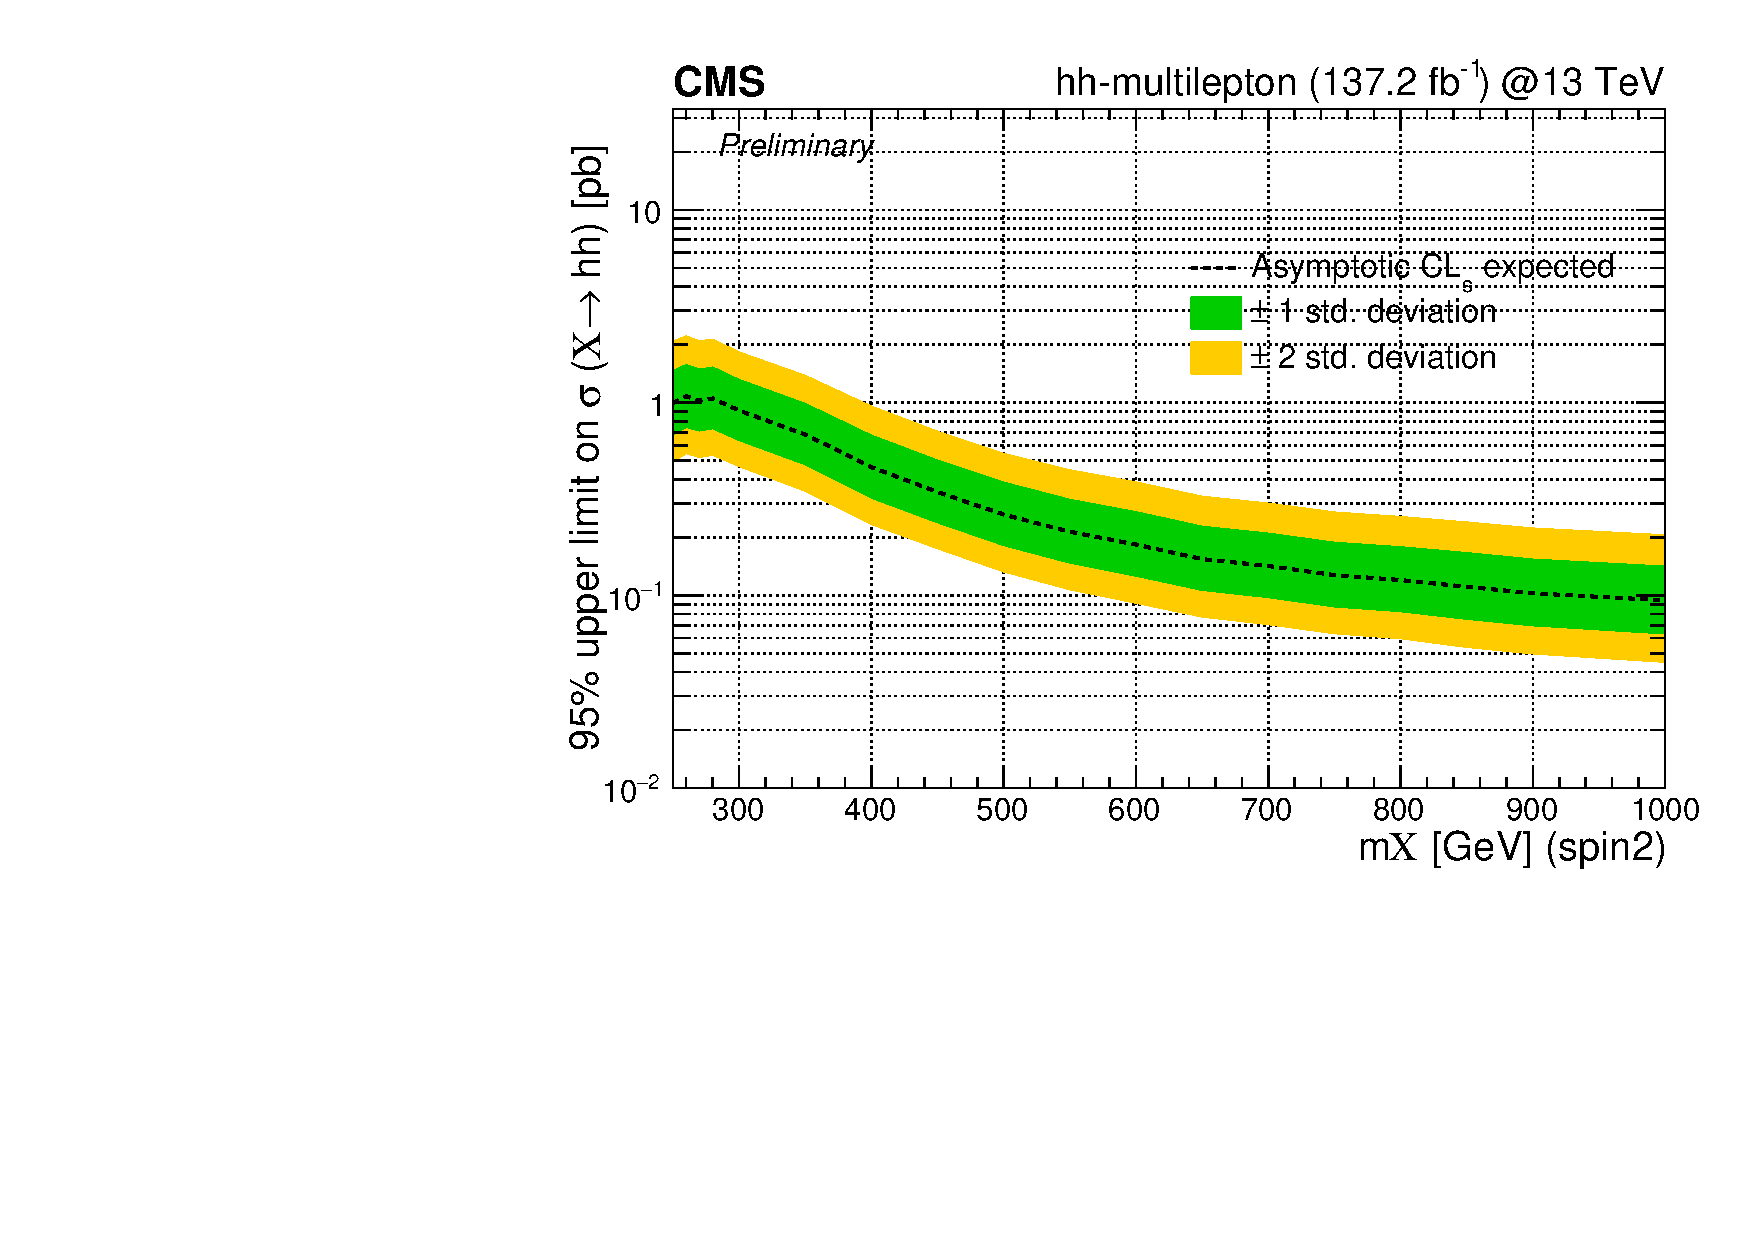
\includegraphics[width=0.45\textwidth]{figures/massScan_spin2_multilepton_RUN2.pdf}
  \hspace{0.05\textwidth}
  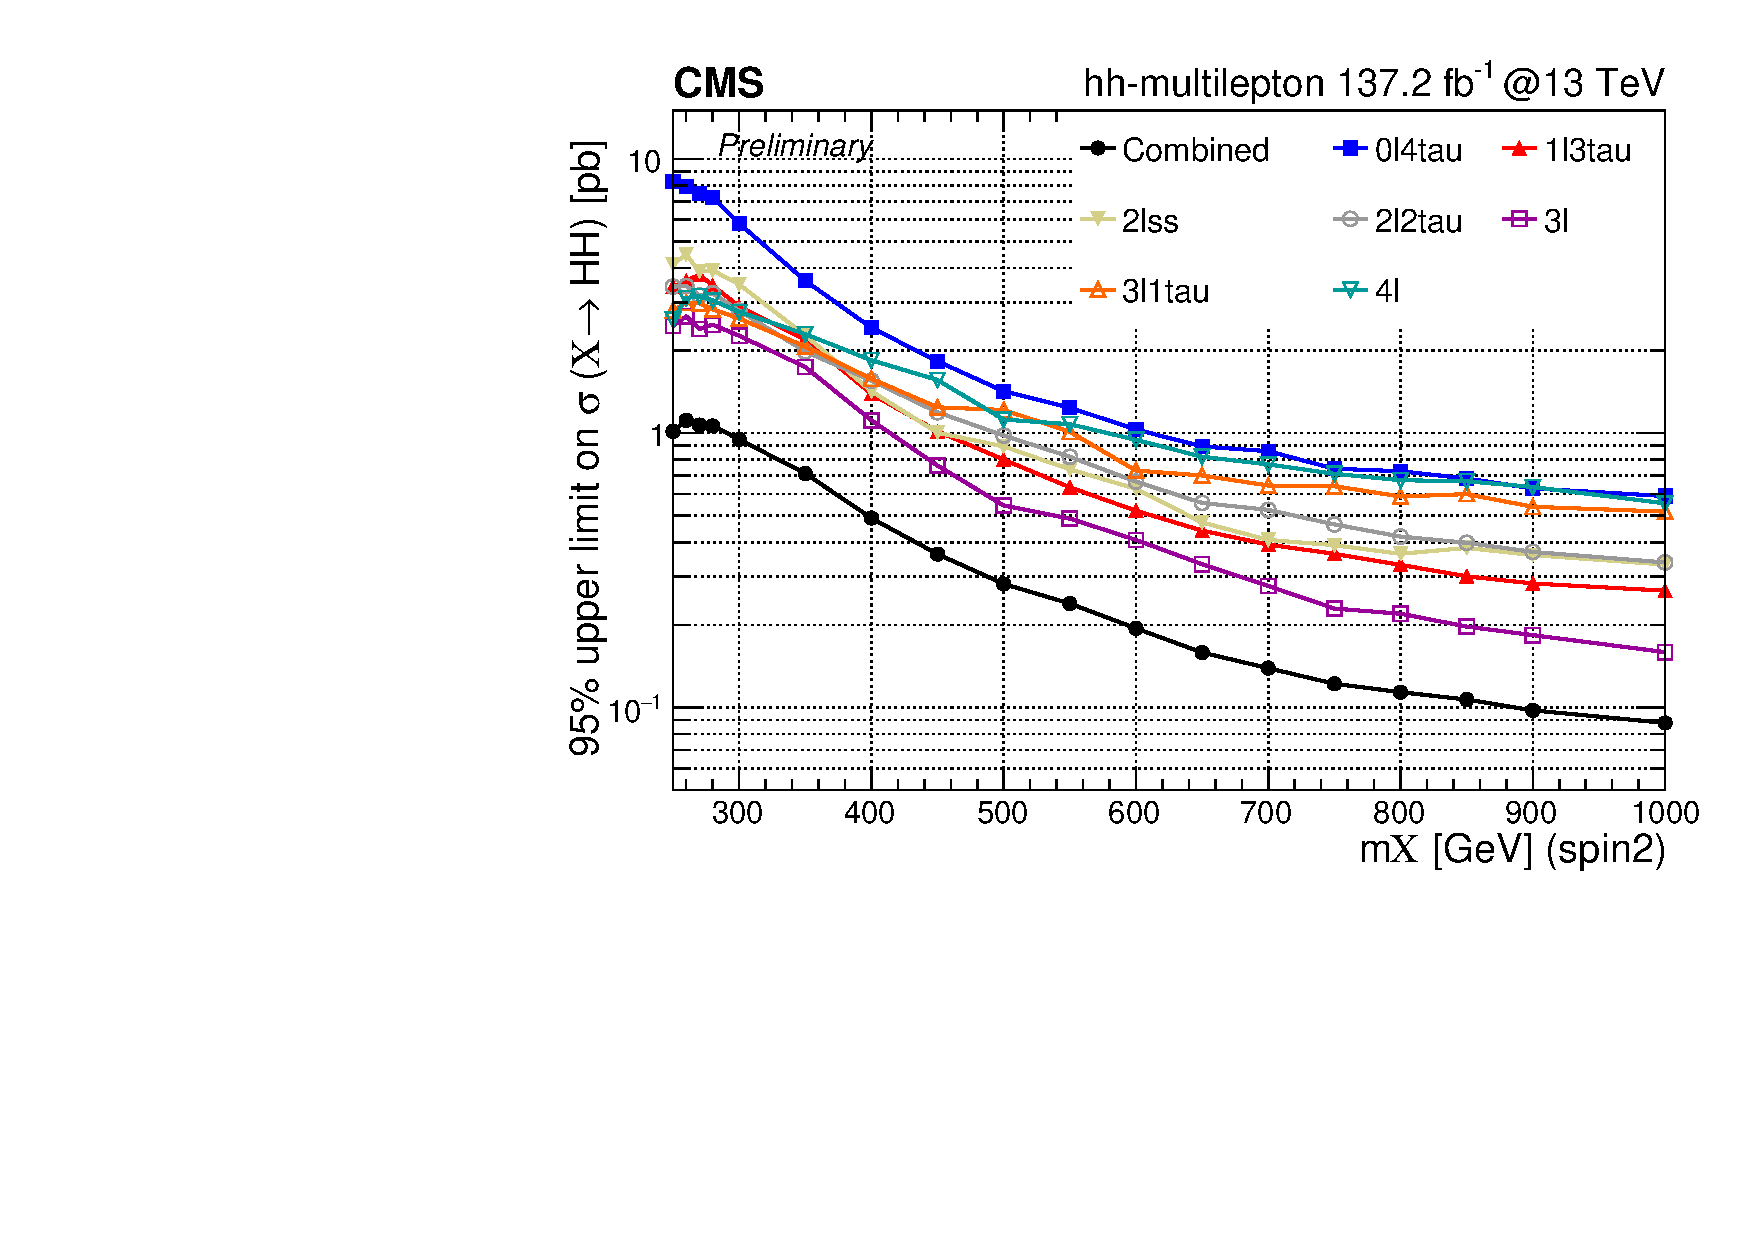
\includegraphics[width=0.45\textwidth]{figures/massMultiScan_spin2_multilepton_Run2.pdf}
  \caption{
    Observed and expected 95\% CL limits on resonant spin-2 $\HH$ production in
    the mass range $250 - 1000\GeV$ for the CMS Run~2 dataset of 137.2\fbinv,
    for the combination of all event categories (left),
    and for each of the seven event categories separately (right).
  }
  \label{fig:HH_limits_spin2}
\end{figure}
